\section{Speech Synthesis Systems}
\label{speec_synthesis_systems}
In this project we will use a HMM-based TTS system, but there are many different speech synthesis systems with their own advantages an disadvantages. In this section we will introduce the general architecture of a TTS system and diverse synthesis methods.

\subsection{TTS Architecture}
The main goal of a TTS system is to synthesize utterances from an arbitrary text. It is easy to notice that synthesizing from a text gives an extra flexibility to a synthesis system but also an extra work has to be done to transform that text into the phonetic units required as inputs by the synthesizer. A general diagram of a TTS system is shown in Figure \ref{fig:tts_architecture}.

\begin{figure}[htb]
	\begin{center}
	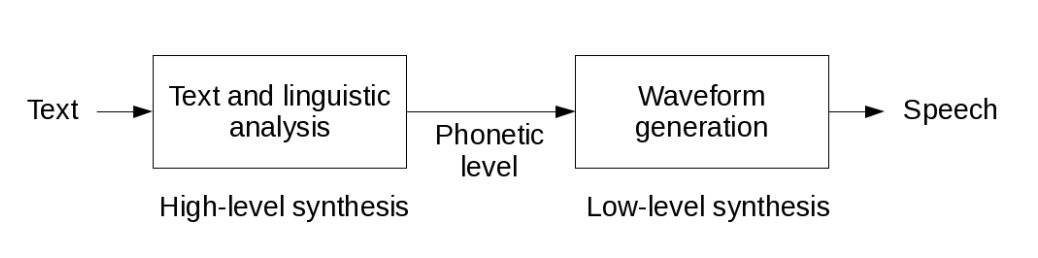
\includegraphics[width=\textwidth]{images/tts_architecture.jpg}
	\caption{General block diagram of a TTS system \cite{TuomoMSc}}
	\label{fig:tts_architecture}
	\end{center}
\end{figure}

The block representing the text and linguistic analysis is what differences a TTS system from other speech synthesis systems. The analysis made to the text has to generate the phonetic representation needed by the next component and predicting the desired prosody. A larger set of goals will imply a more complex text and linguistic analysis. For example, trying to imitate the speaking style used in by sport broadcaster will need an extra function aiming to figure out the style of the input text. 

The main path followed by the text analysis includes a mandatory text normalization module. It is very important to normalize the text before trying to obtain its phonetic representation, to transform numbers, dates, acronyms and all the particularities that a language admit into a standardized form accepted by the system. Also, this module is in charged of defining how similar spelled words are pronounced, e.g. the verb read has to different pronunciations whether is in the present tense or in the past tense. As it can be seen, text normalization is a complex problem that many researchers are looking for a solution to. An interesting approach is discussed in \cite{Sproat2001}.

Once the text is normalized, i.e. converted to plain letters, the structural properties of the text are analyzed and it is converted to a phonetic level. This last conversion is called the letter-to-sound conversion \cite{Pickett1999}. 

When the input text has gone through the first block represented in Figure \ref{fig:tts_architecture}, the low-level block generates predicts, based on the structural information and the prosodic analysis and tipically using statistical models, the fundamental frequency contour and phone durations. Finally, the speech waveform is generated by the vocoder. 

\subsection{Speech Synthesis Methods}
\label{speech_synthesis_systems_methods}
The generation of the waveform can be carried out in several ways, thus, we can talk about different speech synthesis methods. As written in \cite{TuomoMSc}, the different methods can be divided in two categories attending to whether the speech is generated from parameter, i.e. completely artificial, or real speech samples are used during the process. From all the methods explained in this section, only concatenative synthesis uses real samples to synthesize speech.

\subsubsection{Formant Synthesis}
\label{formant_speech_synthesis}
Formant synthesis is the most basic acoustic speech synthesis method. Based on the source-filter theory, which states that the speech signal can be represented in terms of source and filter characteristics \cite{Fant1970}, models the vocal tract with individually adjustable formant filters. The filters can be connected in serial, parallel or both. The different phonemes are generated by adjusting the center frequency, gain and bandwidth of each filter. Depending on the time intervals taken to do the adjustment, continuous speech can be generated. The source is modelled with voice pulses or noise.

Dennis Klatt's publication of the Klattalk synthesizer (see Section \ref{history_vocoder}) was the biggest boost received by formant synthesis. However, nowadays the quality given by this kind of synthesizers is lower than other newer methods, such as concatenative systems. Even so, formant synthesis is used in many applications such as reading machines for blind people, thanks to its intelligibility \cite{Pickett1999}.

\subsubsection{Articulatory Synthesis}
\label{articulatory_speech_synthesis}
The aim of articulatory synthesis is to model the nature speech in the most possible accurate way. Therefore, this is theoretically the best method in order to achieve high-quality synthetic voices. However, modelling the speech as accurately as possible raises the difficulty. The main setbacks are the difficult implementation needed in an articulatory speech synthesis system and the computational load, limiting this technique nowadays. Despite its currently limitations, articulatory models are being steadily developed and computational resources are still increasing, revealing a promising future.

\subsubsection{Concatenative Synthesis}
\label{concatenative_speech_synthesis}
Concatenative method use prerecorded samples of real speech to generate the synthetic speech. It is easy to deduce that concatenative synthesis stands out from other methods of synthesis in terms of naturalness. There are several unit lengths, such as word, syllable, phoneme, diphone, etc, that are smoothly combined to obtain the speech according to the input text. 

The main problem when using concatenative synthesis are the memory requirements. It is almost impossible to store all the necessary data for various speakers and contexts, making this technique the best one to imitate one specific speaker with one voice quality, but also makes it less flexible. It is difficult to implement adaptation techniques to obtain a different speaking style or a different speaker in concatenative speech. Apart from the storage problem, that thanks to the decrease of computer storage and database techniques is becoming less serious, the discontinues found in the joining points may cause some distortion even though the use of smoothing algorithms.

Concatenative systems may be the most widely used nowadays, but due to the limitations before commented, aboce all the flexibility problem, they might not be the best solutions.

\subsubsection{LPC-Based Synthesis}
\label{lpc_based_speech_synthesis}
As in formant synthesis, in LPC-based synthesis utilizes source-filter theory of speech production. However, in this case the filter coefficients are estimated automatically from a short frame of speech, while in formant synthesis the different parameters are found for individual formant filters. Depending on the segment to be synthesized, the excitation needed is either a periodic signal, when synthesizing voiced segments, or noise, in case the segment is unvoiced. 

Linear Prediction (LP) has being applied in many different fields for a long time and was first used in speech analysis and synthesis in 1967. The idea is to predict a sample data by a linear combination of the previous samples. However, LPC targets not to predict any samples, but to represent the spectral envelope of the speech signal. 

Though the quality of basic LPC vocoder is consider poor, using more sophisticated LPC-based methods can produce high quality synthetic speech. The type of excitation is very important in LPC-based systems \cite{TuomoMSc}, but in its accuracy estimating the speech parameters and a relative computational speed lays the strength of LPC-based synthesis.

\subsubsection{HMM-Based Synthesis}
\label{hmm_based_speech_synthesis}
The use of HMMs in speech synthesis is one widely applied method. It is an statistical model used for modelling the speech parameters extracted from a speech database. Once the statistical models are built, they can be use to generate parameters according a text input that will be use for synthesizing. 

HMM-based synthesizers are able to produce different speaking styles, different speakers and even emotional speech. Other benefits are a smaller memory requirement and better adaptability. This last benefit is very interesting to us. While working with noisy data, the less data corrupted by noise used in the system will probably improve the final results. Thus, constructing a high-quality average model and then taking profit of the adaptability of these systems to use the noisy data to adapt the model, because the adaptation data is always much lower than the training data, seems the correct approach.

On the other hand, naturalness is usually lower in HMM-based systems than in other ones, but it must be said that these systems are usually developing very fast. 

As in this project we will be using HMM-based TTS systems, they are going to be described with more detail in Section \ref{hmm_synthesis}.
